% Combine eight of the original poster designs into one document for color proof
% printing. Run `originals.sh` first (from the root directory of the
% repository), then compile this file. Note that this might introduce tiny
% errors depending on which LaTeX engine you use, so you're probably best off
% proofing this document *and* one of the originally generated PDFs before
% committing to a "full" print run.

\documentclass{standalone}
\usepackage{graphicx}

\begin{document}
    
\includegraphics[clip, trim={ 0.0cm   0 18.375cm 0}, width=2.625cm]{../rule30.pdf}%
    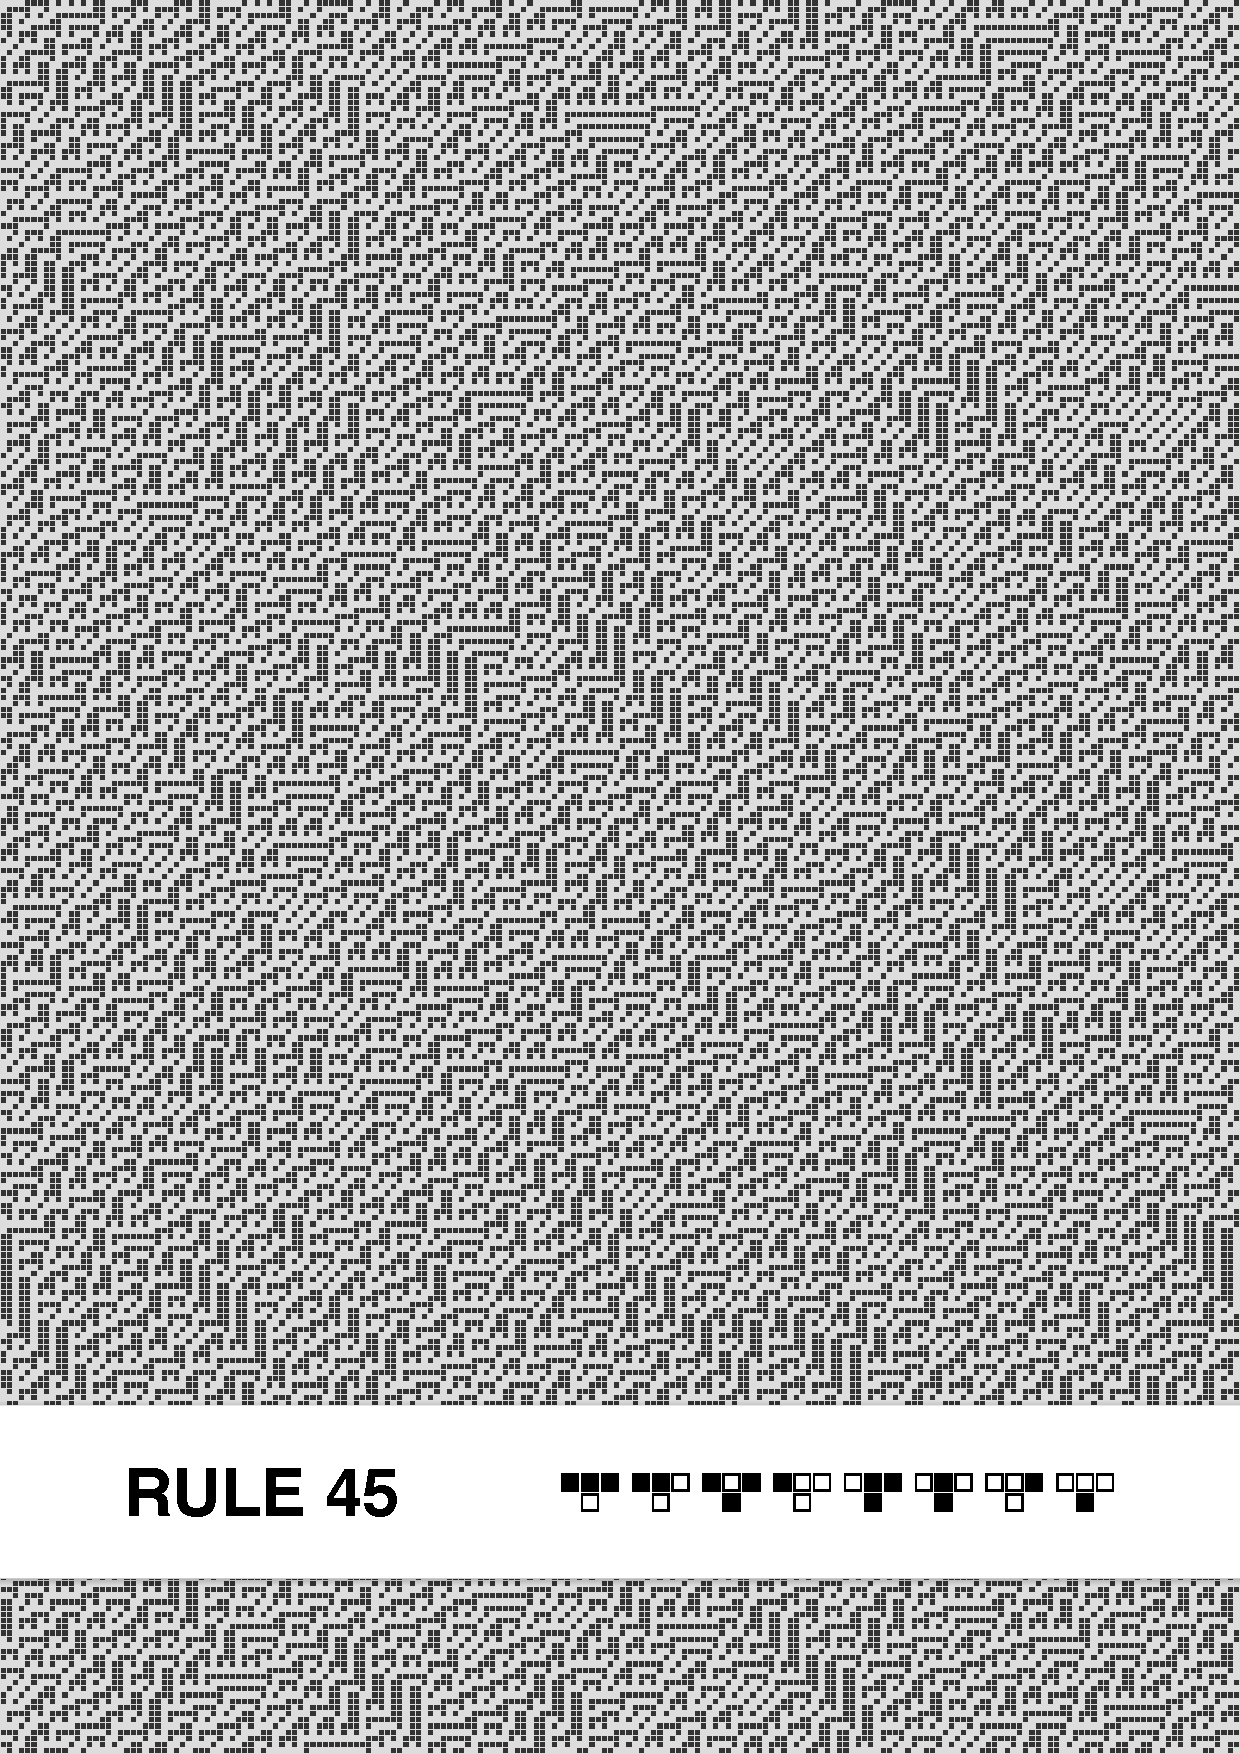
\includegraphics[clip, trim={ 2.625cm 0 15.75cm  0}, width=2.625cm]{../rule45.pdf}%
    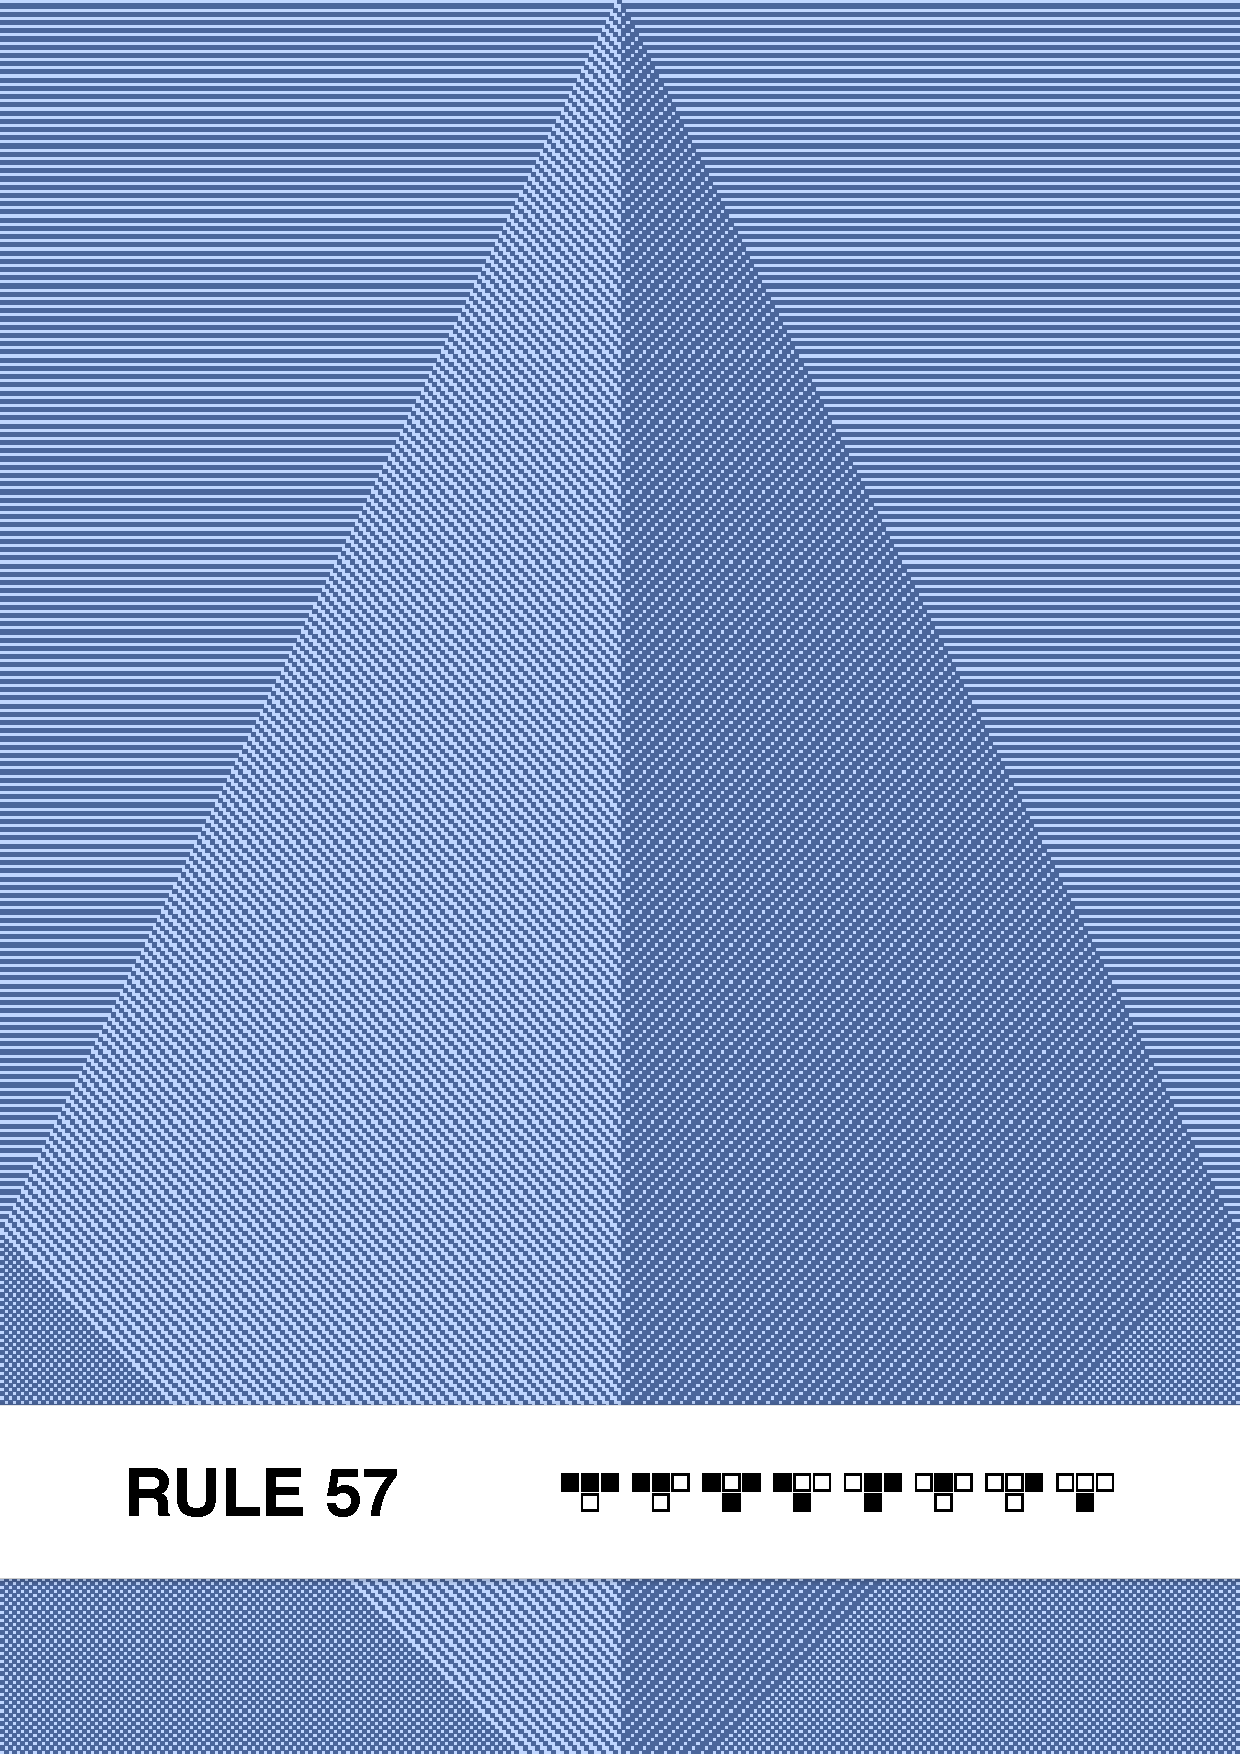
\includegraphics[clip, trim={ 5.25cm  0 13.125cm 0}, width=2.625cm]{../rule57.pdf}%
    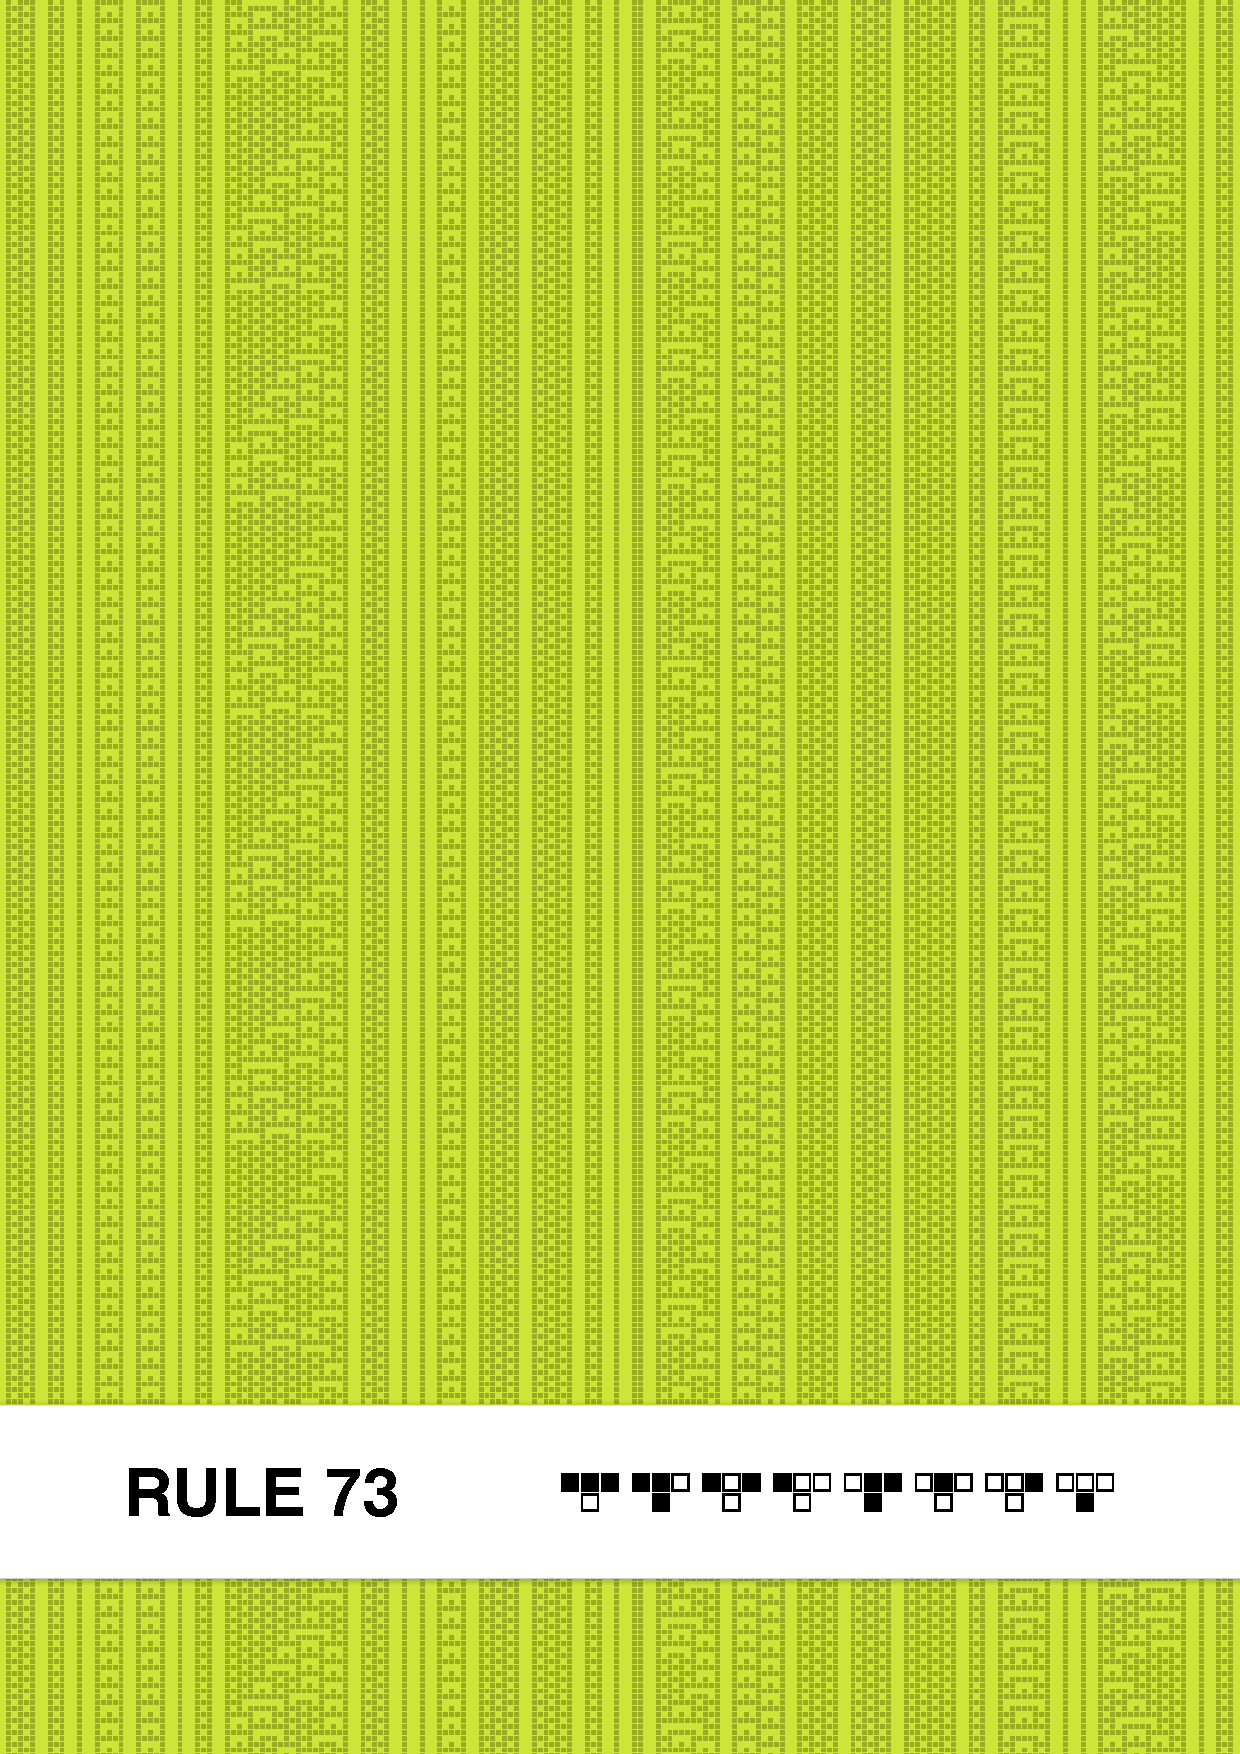
\includegraphics[clip, trim={ 7.875cm 0 10.5cm   0}, width=2.625cm]{../rule73.pdf}%
    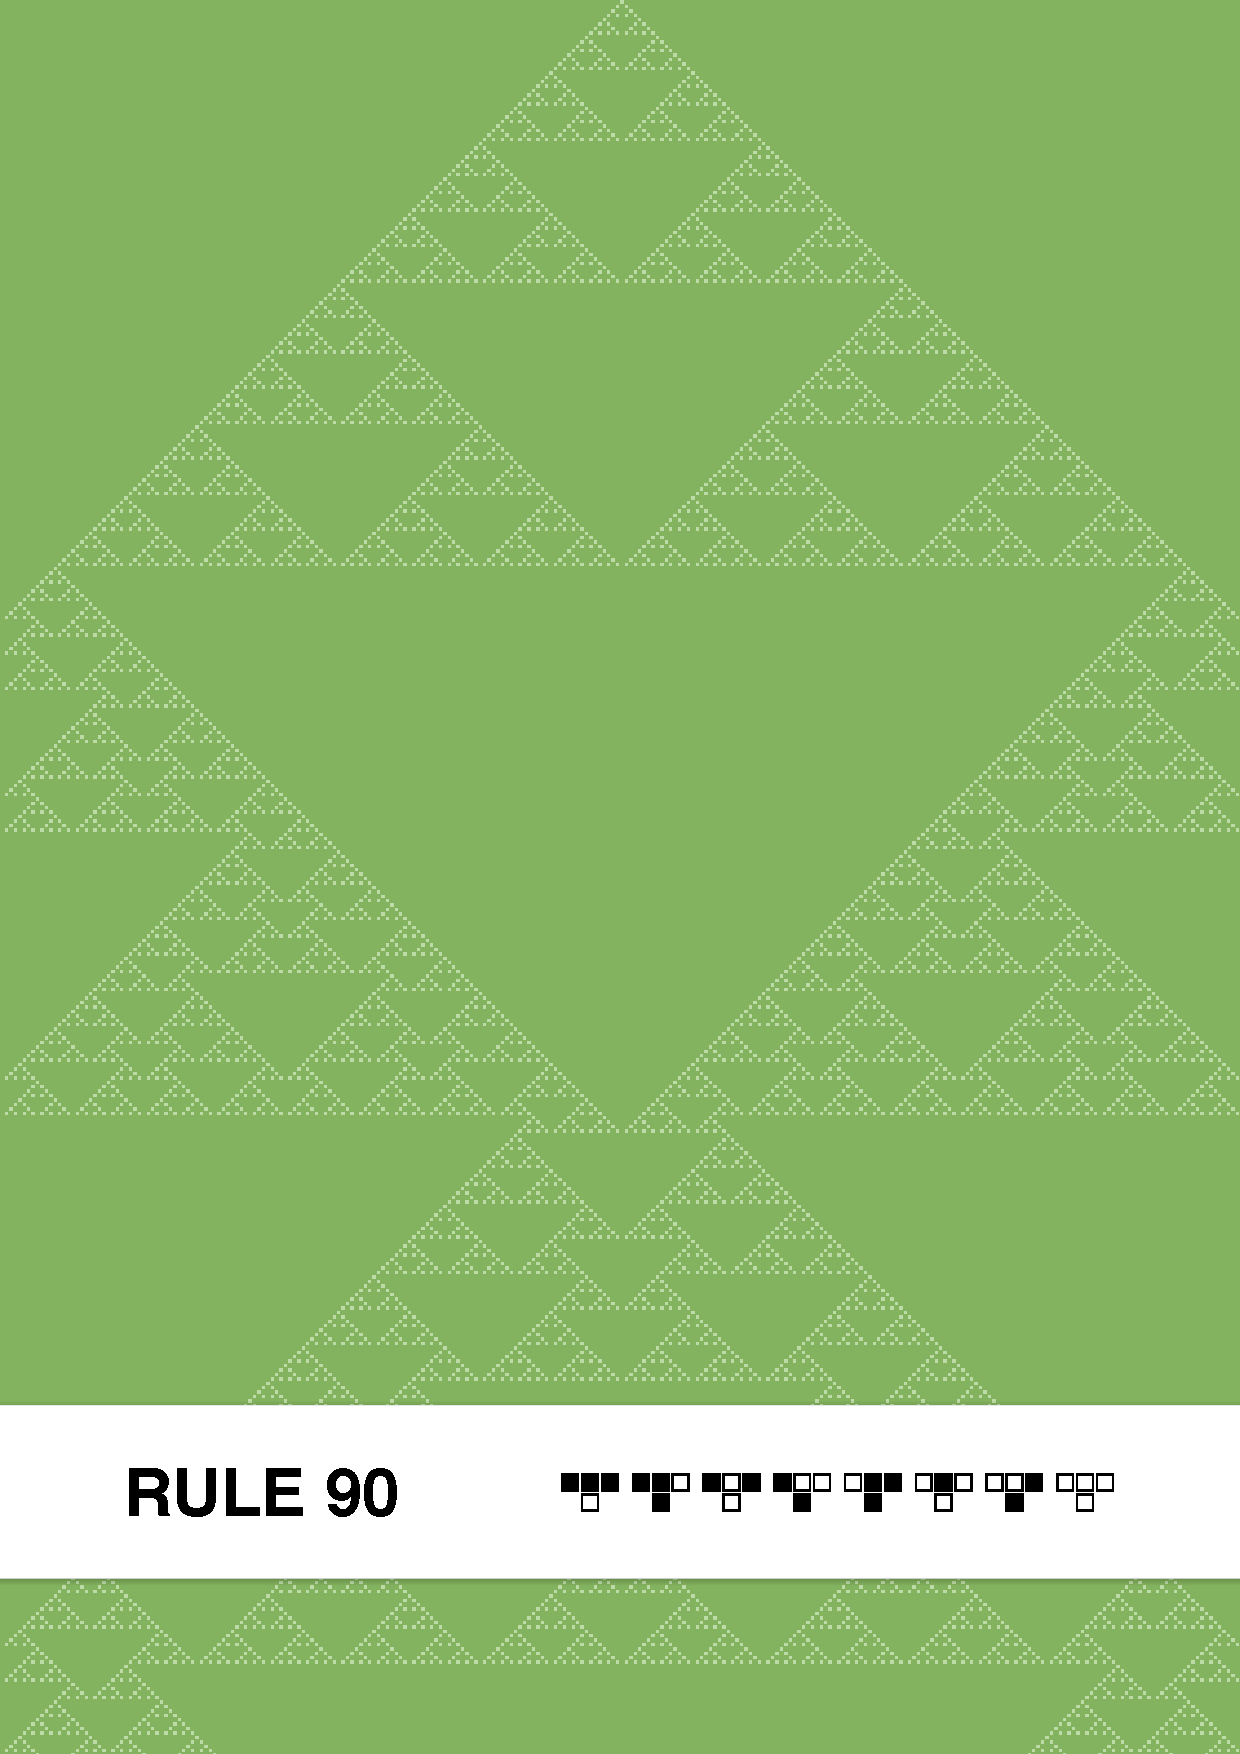
\includegraphics[clip, trim={ 10.5cm  0  7.875cm 0}, width=2.625cm]{../rule90.pdf}%
    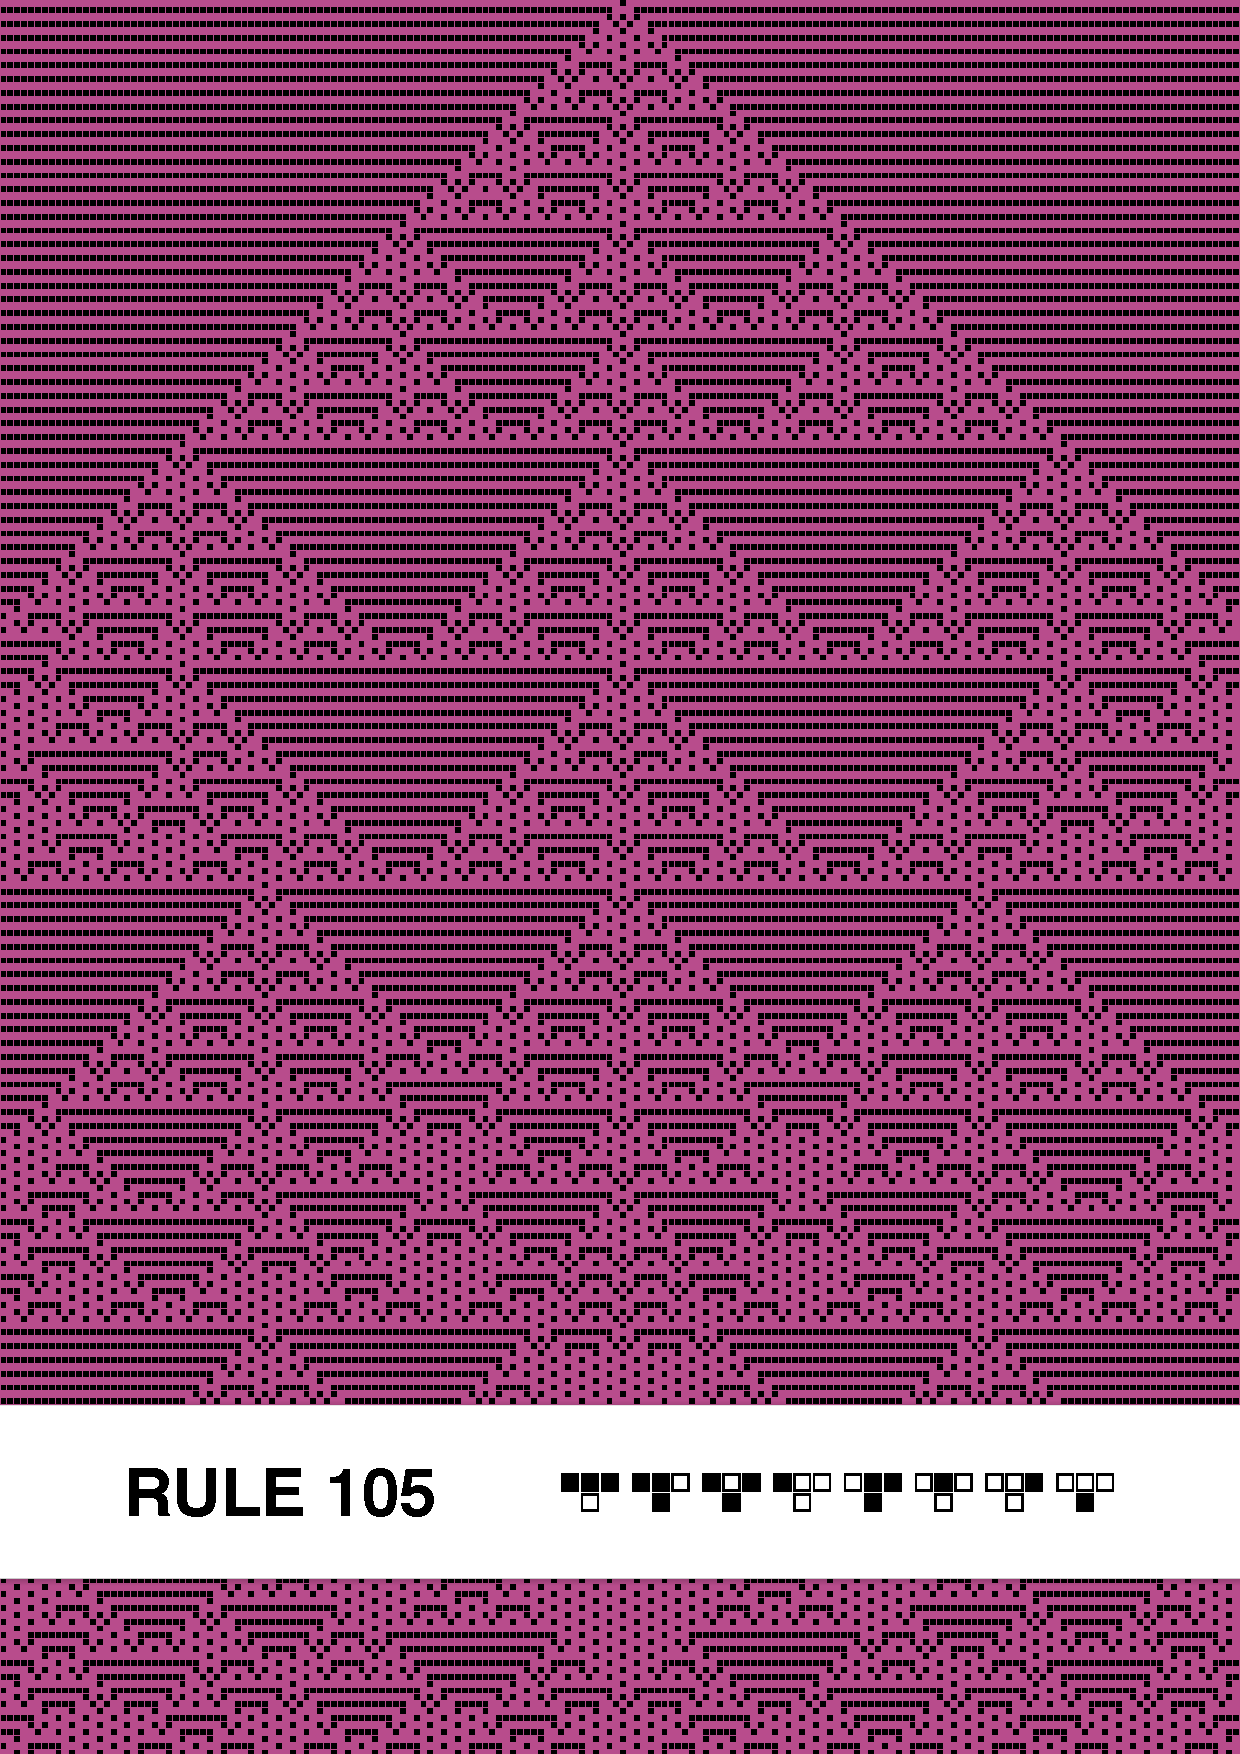
\includegraphics[clip, trim={13.125cm 0  5.25cm  0}, width=2.625cm]{../rule105.pdf}%
    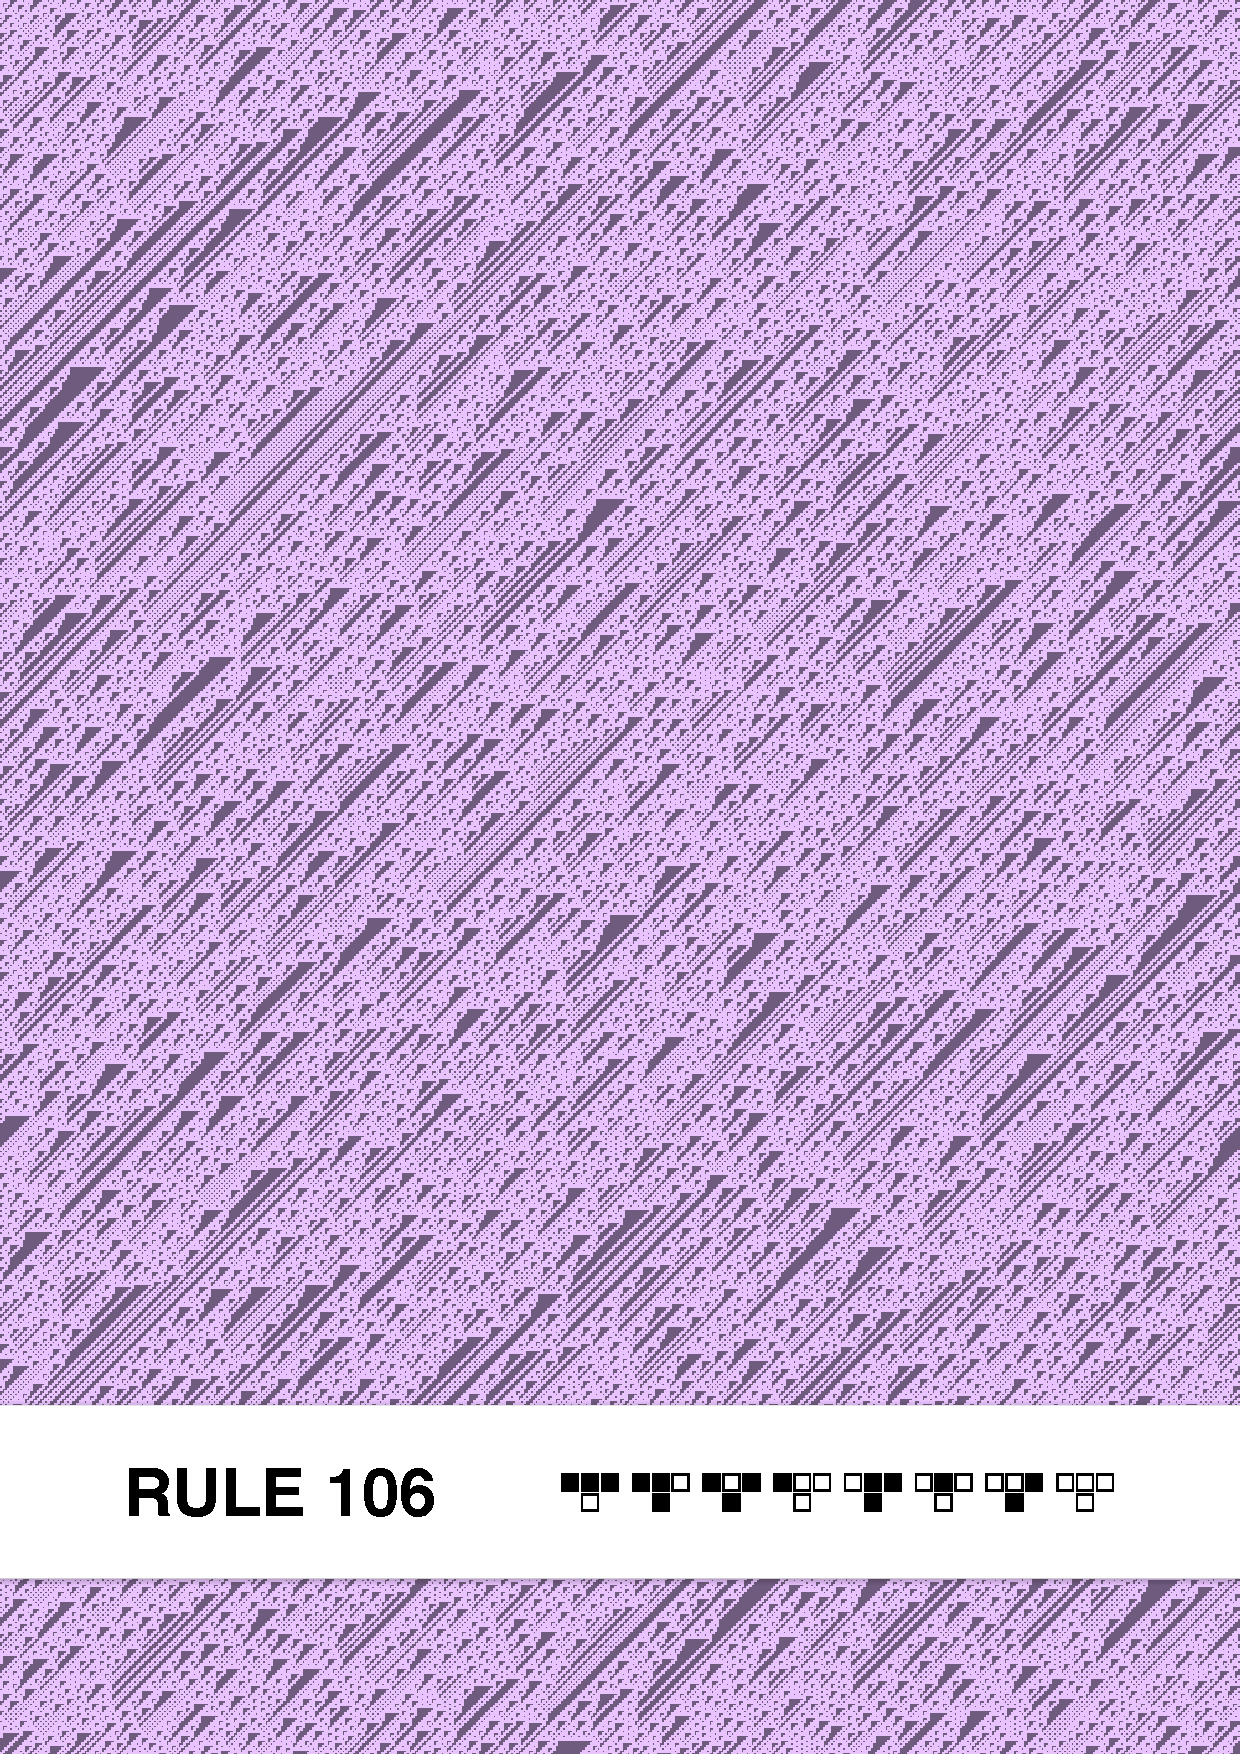
\includegraphics[clip, trim={15.75cm  0  2.625cm 0}, width=2.625cm]{../rule106.pdf}%
    
\includegraphics[clip, trim={18.375cm 0  0.0cm   0}, width=2.625cm]{../rule110.pdf}%
\end{document}
